\documentclass[10pt]{scrartcl}
%
%%%%%%%%%%%%%%%%%%%%%%%%%%%%%%%%%%%%
%% Common preamble
%%%%%%%%%%%%%%%%%%%%%%%%%%%%%%%%%%%%
% PAGE
\usepackage{fullpage} % uncomment this when changing to jour/conf style
% FONTS
\usepackage{lmodern} % enhanced version of computer modern
\usepackage[T1]{fontenc} % for hyphenated characters and textsc in section title
\usepackage{microtype} % some compression
% MATH
\usepackage{amssymb}
\usepackage{listings}
\usepackage{mathtools} % contains amsmath which comes with align
\usepackage{amsthm} % newtheorem stuff
\usepackage{bm} % for bold math (use $\boldsymbol{}$)
% COLOR
\usepackage[usenames,dvipsnames]{color}
%%
% REFERENCING
\usepackage[square,sort&compress,numbers]{natbib} %sorts bibs when they are collectively cited
%%
% TABLES
\usepackage{multirow}
\usepackage{ctable} % provides toprule, bottomrule, midrule
\usepackage{array} % new implementation of tabular & array with lots of enhancements
%%
% FIGURES
\usepackage{graphicx}
\usepackage{grffile} % to set right names of files
%%
% CAPTIONS
\usepackage{caption}
\usepackage{subcaption} % supersedes subfigure & subfloat. try using options
%%
% LISTS
\usepackage{enumitem}
% ALGO
\usepackage[ruled,linesnumbered]{algorithm2e}
%% comments & todo
\newcommand{\comment}[1]{{\color{red}#1}}
\usepackage[colorinlistoftodos]{todonotes}
\newcommand{\TODO}[1]{\todo[inline,color=red!10,size=\small]{#1}}
%% COMMANDS
\newcommand{\comp}[1]{\overline{#1}}  %{\widetilde{#1}}
\DeclareMathOperator{\Var}{Var}
\DeclareMathOperator{\Cov}{Cov}
\DeclareMathOperator{\bigo}{O}
\DeclareMathOperator{\bigom}{\Omega}
\DeclareMathOperator{\davg}{d_{avg}}
\DeclareMathOperator*{\argmax}{arg\,max}
\DeclareMathOperator*{\argmim}{arg\,min}
% Note: \deg is already defined
\newcommand{\expect}{\mathbb{E}}
%
\newcommand{\ceil}[1]{\left\lceil #1 \right\rceil}
\newcommand{\floor}[1]{\left\lfloor #1 \right\rfloor}
%
\newcommand{\reals}{\mathbb{R}}
\newcommand{\field}{\mathbb{F}}
\newcommand{\integers}{\mathbb{Z}}
%
\newtheorem{theorem}{Theorem}[]{\bfseries}{\itshape} 
\newtheorem{lemma}[theorem]{Lemma}{\bfseries}{\itshape}
\newtheorem{claim}[theorem]{Claim}{\bfseries}{\itshape}
\theoremstyle{definition}
\newtheorem{definition}[theorem]{Definition} % {\bfseries}{\itshape}
\newtheorem{observation}[theorem]{Observation} % {\bfseries}
\newtheorem{condition}[theorem]{Condition} % {\bfseries}{\itshape}
\newtheorem{note}[theorem]{Note} % {\bfseries}{\itshape}
% ROMAN NUMERALS
\makeatletter
\newcommand{\rmnum}[1]{\romannumeral #1}
\newcommand{\Rmnum}[1]{\expandafter\@slowromancap\romannumeral #1@}
\makeatother
% TWO VERSIONS
%% \usepackage{etoolbox}
%% \newtoggle{withappendix}
%% \toggletrue{withappendix} % comment this if you want journal version
%% Usage: iftoggle{withappendix}{}{}
%%
%% math operator
%% \DeclareMathOperator{\sgn}{sgn}
% CODEBOX
%% \usepackage[framemethod=tikz]{mdframed}
%% \newmdenv[linecolor=black!10,innerlinewidth=0pt, roundcorner=4pt,innerleftmargin=6pt,
%% font=\ttfamily,innerrightmargin=6pt,innertopmargin=6pt,
%% innerbottommargin=6pt,backgroundcolor=black!10]{codeblock}
%%%%%%%%%%%%%%%%%%%%%%%%%%%%%%%%%%%%
%% preamble ends
%% from now on, draft specific
%%%%%%%%%%%%%%%%%%%%%%%%%%%%%%%%%%%%
%% \RequirePackage[l2tabu, orthodox]{nag}
%%
\title{PatchSim Model Description}
\author{Srini Venkatramanan\footnote{Email:vsriniv@bi.vt.edu}}
\begin{document}
\maketitle

Mechanistic approaches to disease simulation often fall under one of two 
categories: 
\begin{itemize}
	\item \textbf{ODE models} Approaches of this kind are based on ordinary 
	differential equations with the central assumption being \emph{homogeneous 
	mixing} of individuals within the population of interest. While easy to 
	setup and simulate, they often cannot reproduce spatial or social 
	heterogeneity observed in the ground truth.
	
	\item \textbf{Network models} Approaches of this kind simulate the disease 
	dynamics on a graph (e.g., social network)
	where disease propagates from infected to susceptible individuals through 
	the edges of the graph, capturing social interactions. They can be 
	implemented in an agent-based manner and allow for high fidelity of 
	representation. However, such models are tough to setup and pose 
	computational challenges in model simulation and calibration. 
\end{itemize}

Metapopulation models take advantage of both these approaches, and are well 
suited to capture spatial heterogeneity in disease dynamics. The population of 
interest is divided into spatially distinct \emph{patches}, and within each 
patch the disease dynamics are simulated with a homogeneous mixing assumption. 
The patches are also connected to each other through a weighted directed 
network capturing movement of individuals between the patches. The movement is 
often representative of \emph{commuting} (as against \emph{migration}), thus 
preserving the home population counts of each patch. While within a single 
patch the disease evolution resembles a homogeneous ODE model, the mobility 
network generates heterogeneity and longer hops between the spatial 
sub-populations. PatchSim is a deterministic implementation of this approach. 

Let $\mathcal{N}$ represent the set of all patches (with $N = |\mathcal{N}|$). 
Associated with each patch $i$, we have population $P_i$, and state tuple 
$Z_i(t)$ denoting number of individuals in each of the disease states at time 
$t$. For a typical SEIR (Susceptible $\to$ Exposed $\to$ Infected $\to$ 
Recovered) model, the set of states is given by $\mathcal{Z} = \{S,E,I,R\}$. 
The state tuple is then $Z_i(t) = (S_i(t), E_i(t), I_i(t), R_i(t))$, with 
$\sum_{z\in\mathcal{Z}} z_i(t) = P_i$. Between a pair of patches $i$ and $j$, 
we have the flow $F_{ij}$, denoting the fraction of individuals belonging to 
\emph{home} patch $i$ spending their day in \emph{away} patch $j$. In order to 
conserve patch populations (i.e., commuting model), we assume $\sum_{j \in 
\mathcal{N}}F_{ij} = 1$. The mobility is assumed to be \emph{homogeneous} and 
\emph{memory-less}, i.e., the commuting individuals according to $F_{ij}$ are 
assumed to be picked at random from the population $P_i$ independent of their 
disease state, and independently for each day of the simulation. Due to the 
movement of individuals, the \emph{effective} population of patches may differ 
from their home population $P_i$. This in turn also affects the state tuple 
$Z_i$. We denote the effective population as $P_i^{\mathtt{eff}}$ and the 
effective state tuple as $Z_i^{\mathtt{eff}}(t)$. Then, $P^{\mathtt{eff}}_i = 
\sum_{k\in \mathcal{N}} F_{ki} P_i$ and  $z^{\mathtt{eff}}_i = \sum_{k\in 
\mathcal{N}} F_{ki} z_i$ for $z\in \mathcal{Z}$. 

PatchSim steps through the disease simulation in daily epochs. In order to 
compute the change in state tuple $\Delta Z(t) = Z(t+1) - Z(t)$, it 
incorporates (i) movement of individuals from their respective home patches to 
away patches according to $F_{ij}$, (ii) exposures, infections, and recoveries 
happening in the away patches, and (iii) integration of state updates at the 
home patches. Let $\beta$ represent the probability of exposure per day per 
$S-I$ contact, $\alpha$ the infection rate and $\gamma$ recovery rate. $\alpha$ 
can be thought of as the reciprocal of mean incubation period, and $\gamma$ the 
reciprocal of mean infectious period. Additionally, let $X_i(t)$ represent the 
spatio-temporal seeding profile. This captures the number of individuals of 
patch $i$ who are extraneously moved from $S$ to $E$ to indicate external 
exposure (`seed' cases). The state update equations can then be written down as 
below for each $z\in\mathcal{Z}$ (omitting time index $t$ for clarity):

\begin{eqnarray}
	\centering 
	\Delta{S}_i &=&  - X_i - \sum_{j \in \mathcal{N}} F_{ij} \beta 
	\frac{I^{\mathtt{eff}}_j}{P^{\mathtt{eff}}_j} S_i \label{eqn:new-exp}\\
	\Delta{E}_i &=& X_i + \sum_{j \in \mathcal{N}} F_{ij} \beta 
	\frac{I^{\mathtt{eff}}_j}{P^{\mathtt{eff}}_j} S_i - \alpha E_i \\
	\Delta{I}_i &=& \alpha E_i - \gamma I_i \\
	\Delta{R}_i &=& \gamma I_i 
\end{eqnarray}

The summation in Equation~\ref{eqn:new-exp} captures new exposures for 
individuals with home patch $i$, summed across potential away patches $j$. 
$F_{ij}$ denotes the movement to away patch $j$, 
$\frac{I^{\mathtt{eff}}_j}{P^{\mathtt{eff}}_j}$ is the proportion of infectious 
individuals in the effective population at patch $j$, and $\beta$ the 
probability of exposure given contact. Note that, unlike exposure, becoming 
infectious ($E \to I$) and recovery ($I \to R$) are independent of the away 
patch $j$ visited by an individual, hence need not be explicitly summed across 
$j \in \mathcal{N}$. 

Thus, given the disease parameters $(\beta,\alpha,\gamma)$ and a seeding 
profile $X$, PatchSim uses the population vector $P$ and flow matrix $F$ to 
produce the spatio-temporal evolution of disease states $Z$.

\begin{figure}
\centering
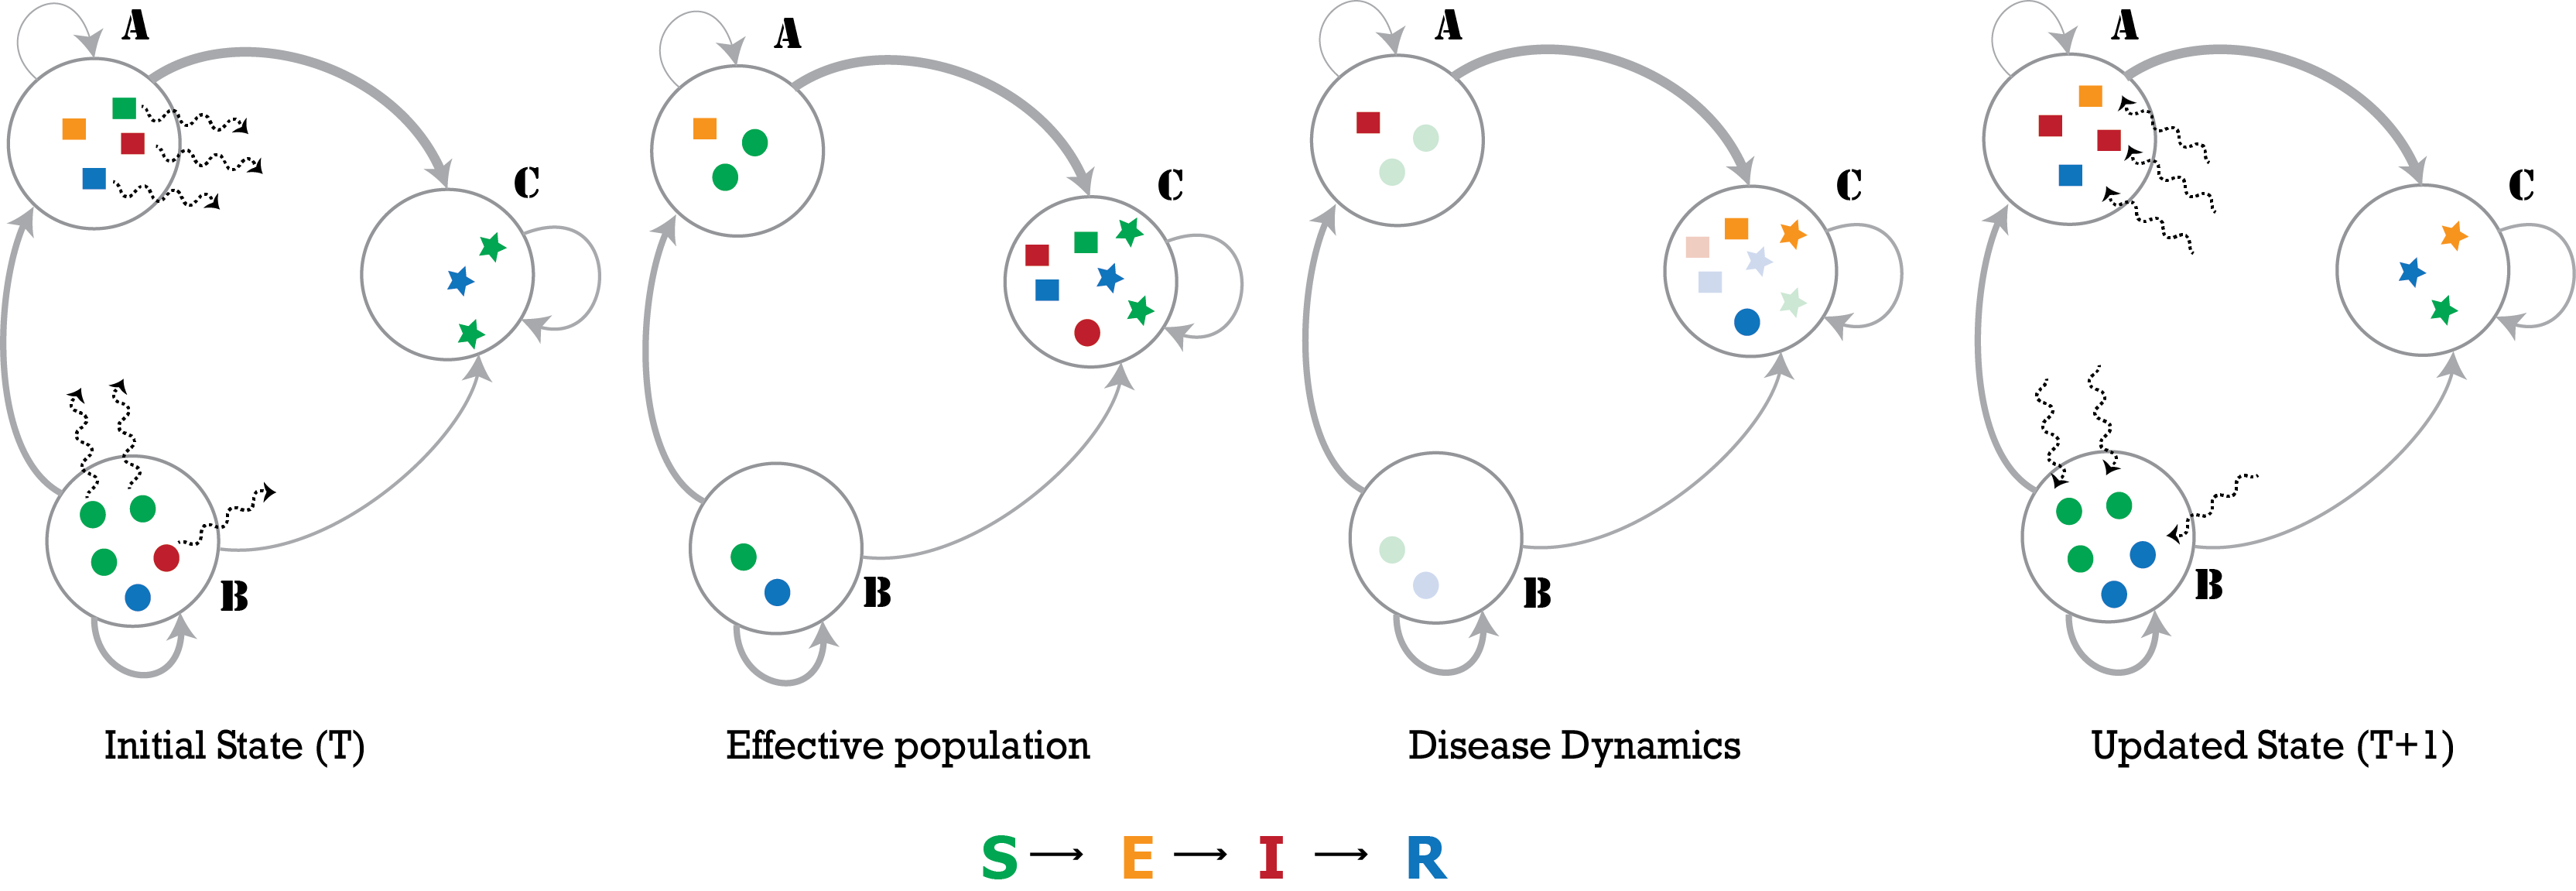
\includegraphics[width=\textwidth]{PatchSim.png}
\caption{The large circles represent the patches in the simulation, and the 
grey edges represent the travel network, with varying thickness denoting 
heterogeneity in flow volumes. The sample population shows 4 individuals in 
patch A (squares), 5 in patch B (circles) and 3 in patch C (stars). The colors 
represent the disease state the individuals are in (susceptible, exposed, 
infected or recovered).  The wavy dashed arrows show movement of individuals 
(randomly chosen according to outgoing edge probabilities). In the first step, 
individuals are moved from their home patch to another patch (first panel), 
creating the effective population (second panel). The disease dynamics may 
constitute an exposure event (transition from S to E), onset of infectiousness 
(E to I), or recovery event (I to R).  The nodes undergoing these transitions 
are highlighted in third panel, where we see an onset of infectiousness in 
patch A, two exposures and a recovery in patch C. Finally, the individuals 
return to their home patch (fourth panel). }
\end{figure}

\end{document}


